\toclesssection{SCP 022 - The Morgue}
\addcontentsline{toc}{section}{SCP 022 - The Morgue}

\textbf{Item \#:} SCP-022

\textbf{Object Class:} Euclid

\begin{figure}[h]
\begin{center}
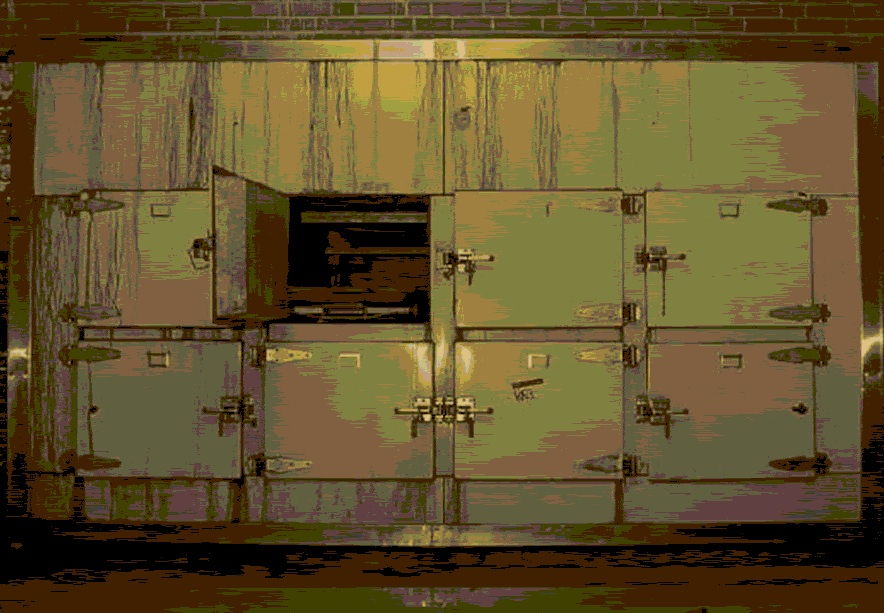
\includegraphics[scale=0.4]{scp/022.jpg}
\linebreak Image of SCP-022 through security camera.
\end{center}
\end{figure}

\textbf{Special Containment Procedures:} A vault door has been installed following Incident 022-827 to seal SCP-022. It is to remain locked at all times, with the sole exception being the appearance of an instance of SCP-022-1. The original door to SCP-022 was destroyed during Incident 022-827, with attempts at replacement being met with failure. Security cameras have been installed to monitor for instances of SCP-022-1.

In the event that an instance of SCP-022-1 appears, automated systems should incinerate it the moment it leaves SCP-022. At this point the vault door may be unlocked to admit cleanup crews. Should the automated systems fail to destroy the instance of SCP-022-1, response teams are cleared to enter and neutralize it. Under no circumstances may any living human enter SCP-022 except at the order of Class-4 personnel for testing purposes. Class-4 personnel may also order instances of SCP-022-1 to be captured and held; however, they may not be removed from SCP-022 containment facilities.

\textbf{Description:} SCP-022 is a morgue in the basement of [REDACTED] Hospital in Great Britain. Until 198\censor{X}, there were no reported anomalous occurrences within the morgue. Reports of strange activity were first received in November of 198\censor{X}. The area was soon quarantined by the Foundation, with an official story being released that the entire building had been condemned. The reason for the sudden manifestation of its strange properties remains under investigation.

Periodically, a random drawer within the morgue will open to reveal a cadaver under a covered sheet. After approximately six minutes open, the cadaver will animate and attempt to leave the morgue. At this point, the cadaver is given the designation SCP-022-1. In some cases the cadaver will be too damaged or decomposed to successfully exit SCP-022 or even rise from the table it lies on. In this case, SCP-022-1 will typically struggle and twitch on the table until expiration occurs. Should an instance of SCP-022-1 expire while remaining on the table, the table slides back into the drawer, which then shuts. Reports indicate that the scent of burnt tissue is evident immediately following such an event.

The energy source that sustains instances of SCP-022-1 is currently unknown. Instances do not breathe, eat, or sleep, and their bodies produce no heat. Analysis of SCP-022-1 following expiration has discovered no abnormal organs or chemicals present; they appear to be fully human cadavers.

Instances also possess physical strength that exceeds that of normal humans. Though direct testing has proven problematic, researchers estimate the strength increase to be approximately 500 N (112 lb) of lifting force greater than what one would expect of a human body sharing a similar condition. Analysis is underway to determine if this effect is connected to the unknown power source or if it is an entirely separate phenomenon.

When body parts are severed from SCP-022-1, the portion with the greatest mass retains its effects; all other pieces become inert. Destruction of the head or brain does not neutralize SCP-022-1; instead, the lower torso and limbs remain animate. Complete tissue destruction appears to be the only method of successfully terminating instances of SCP-022-1. Left alone, instances of SCP-022-1 will simply expire; all motion ceases and they appear to become normal cadavers again. The amount of time this takes depends on how damaged the body is and the rate of decomposition, and can take anywhere between two days and three weeks.

Investigation has revealed that the bodies acting as SCP-022-1 match the description of cadavers reported to have been stolen from morgues across the country. The mechanism for this transfer is currently being researched.

Adding any new matter to SCP-022 has thus far proved impossible. Any object that enters SCP-022 disappears shortly after passing through the door, leaving no trace. This includes inanimate objects and biological specimens. \textbf{See Addenda 022-001 and 022-002}.

So long as an instance of SCP-022-1 possesses a functioning mouth, tongue, and trachea, it is able to communicate fully with researchers. See Interview Log 022-751 for details.
\newpage
\textbf{Addendum 022-001:} A request has been submitted to create a new entrance to SCP-022 by removing a portion of the South wall. Request pending approval.

\textbf{Addendum 022-002:} A pile of matter was discovered on the floor of the room directly above SCP-022. It appeared to contain all matter that had been sent into SCP-022, with the exception of humans. All materials appeared broken and worn down. Metallic components were covered in large amounts of rust, with all biological parts being in various stages of decomposition. Testing revealed that the time between inserting an object into SCP-022 and it reappearing above to be precisely 183 seconds. Humans who enter, however, do not appear in said pile. Instead, humans appear to become integrated into the morgue, and may later animate as instances of SCP-022-1.